It has been over half a century since astrophysicist Sjur Refsdal
first developed the theory to enable the use of a gravitationally
lensed supernova (SN) resolved into multiple images as a cosmological
tool. The first multiply-imaged core-collapse (CC) and Type Ia SN,
Refsdal \citep{Kelly:2015a} and iPTF16geu \citep{Goobar:2016}
respectively, have been discovered in just the past 3 years. As the
light for each of the multiple images follows a different path through
the expanding universe and through the lensing potential, the SN
images appear delayed by hours (for galaxy-scale lenses) or years (for
cluster-scale lenses). These gravitational lenses are also important
tools for extending our SN sample into the early universe, beyond the
limit of current detections at $z\simeq2$. As PI on an ongoing HST
Archival Research Grant, \textbf{I am developing the first open-source
software for analysis of lensed SNe} (\textit{Supernova Time Delays}
[SNTD]).  This Python package will be essential for precise
measurements of lens properties and time delays from the hundreds of
multiply-imaged SN observations expected over the next decade (Figure
1), and despite its design for SNe will be valuable for lensed quasar
measurements as well. My research will have two major components:
1. Using SNTD and multiply-imaged SN as a cosmological
probe. 2. Observing and understanding the rates and physical
properties of very high-z SNe.

\begin{wrapfigure}{r}{.5\textwidth}
\centering
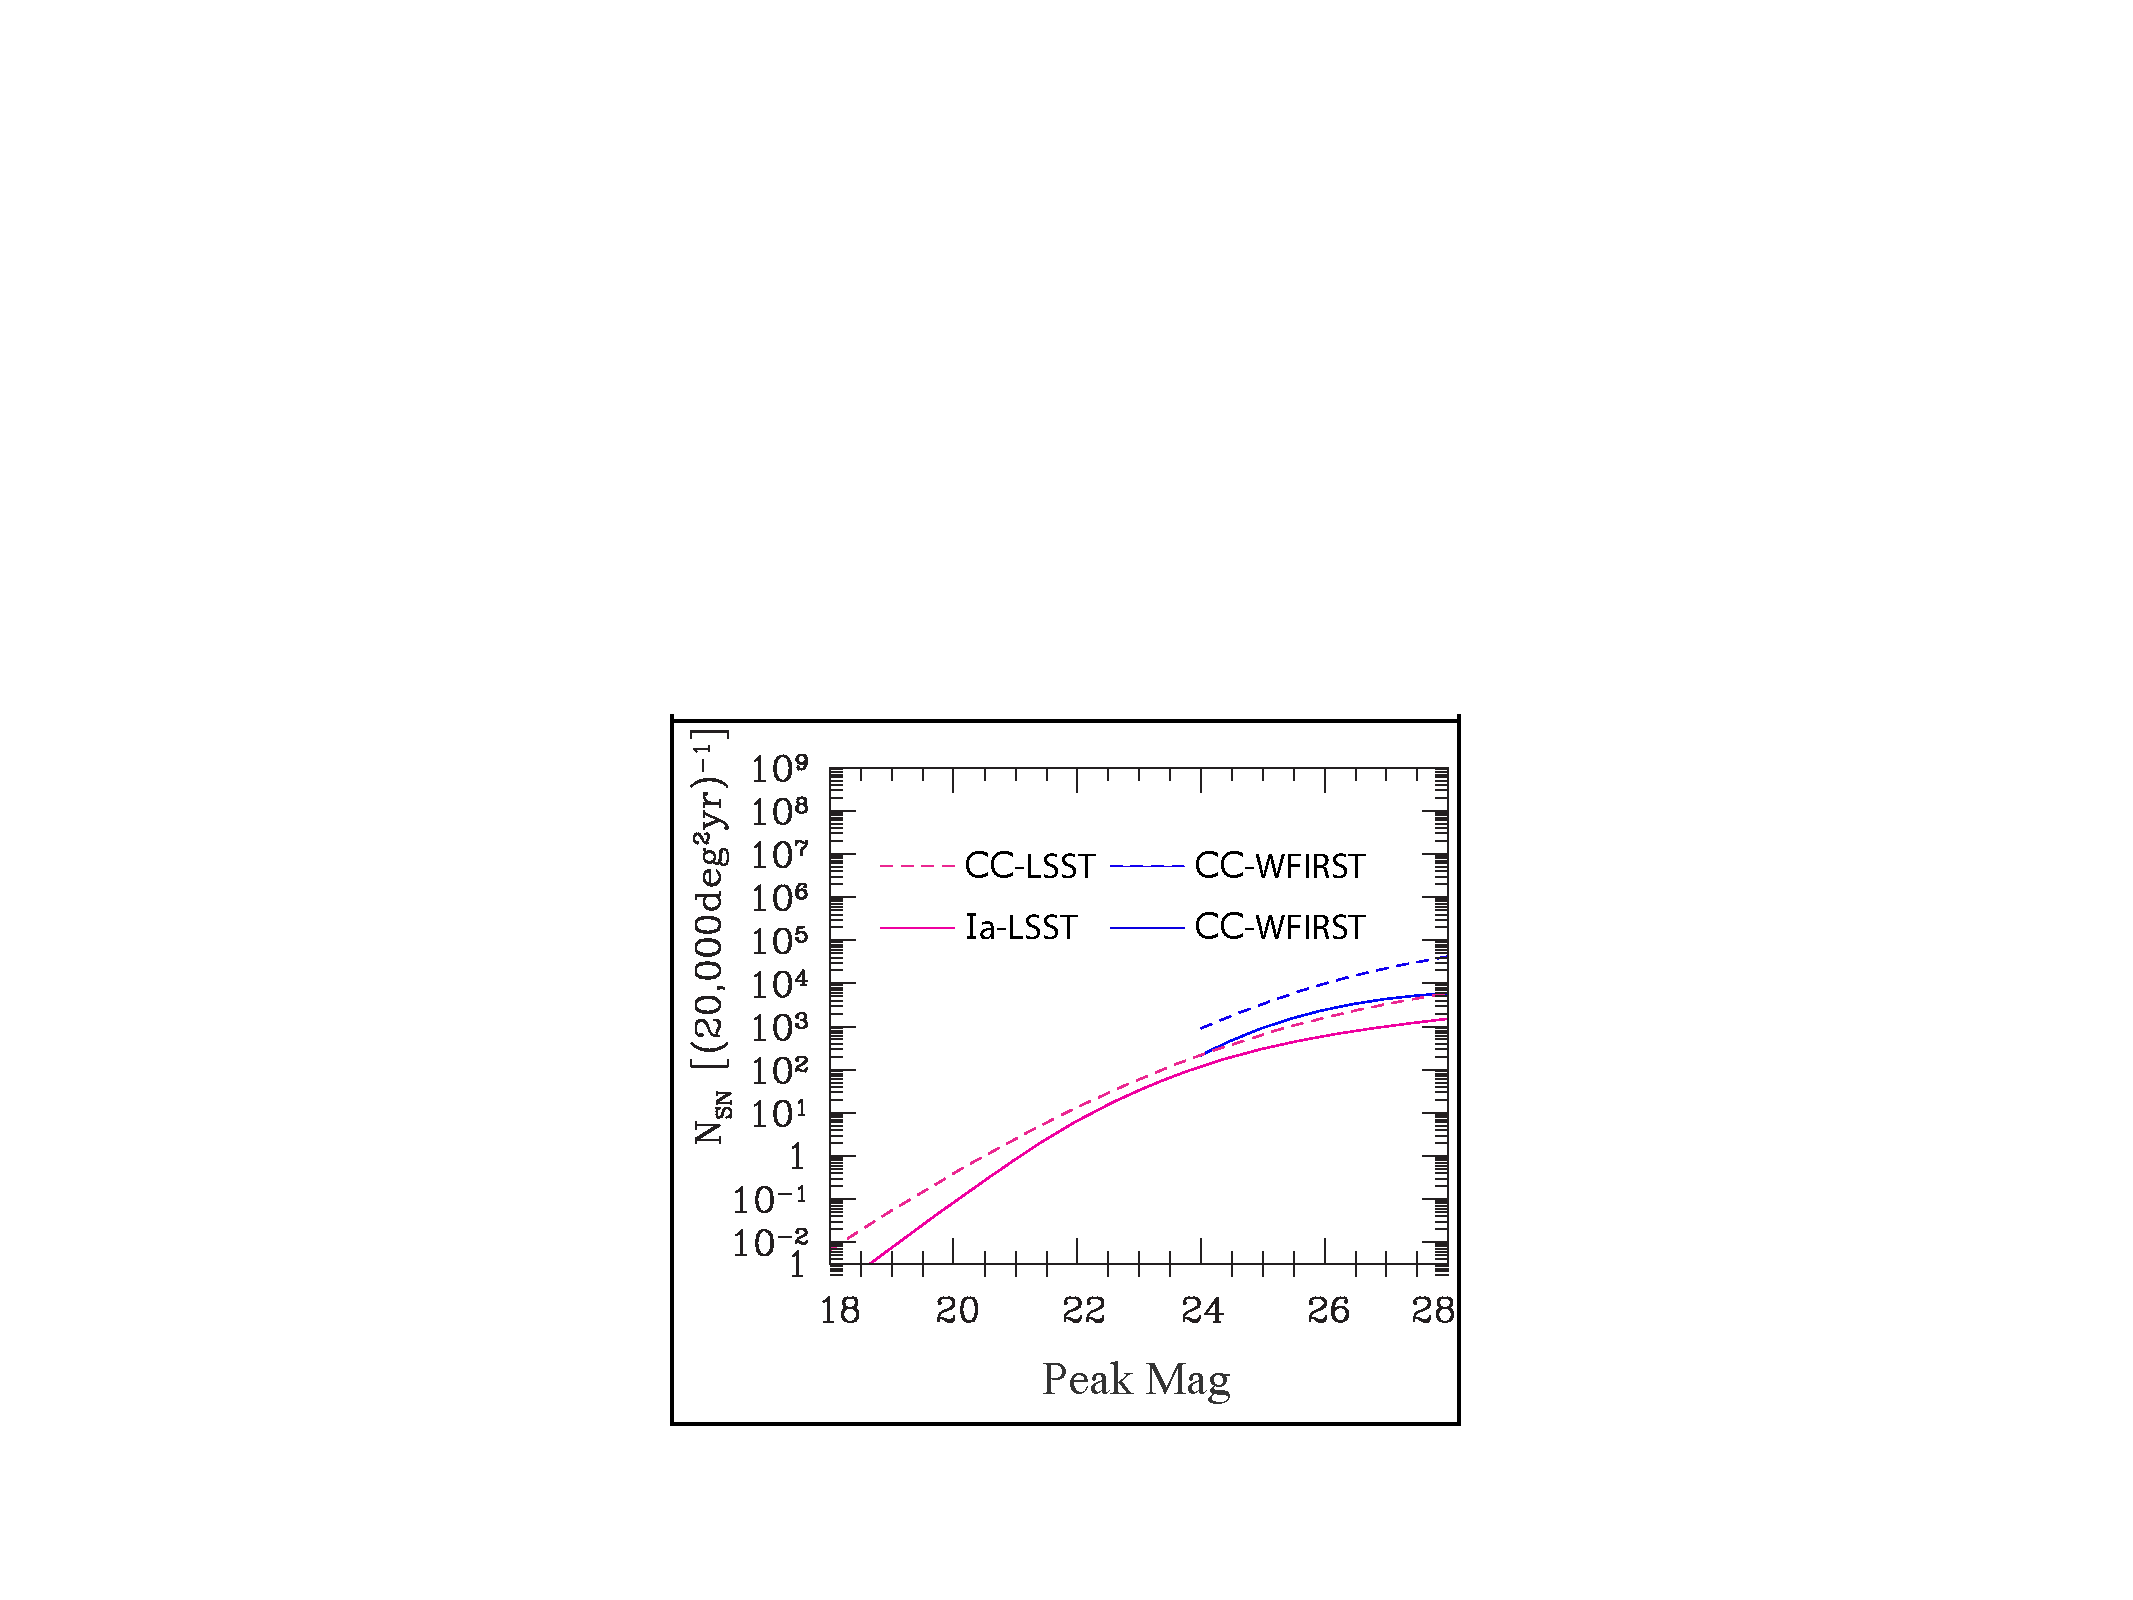
\includegraphics[height=.4\textwidth]{FIG/wfirst_lsst}
\caption{
\noindent\fontsize{10}{14}\selectfont
Expected numbers of lensed SN Ia and Core Collapse SN for LSST
$(i_{peak,lim})$ and WFIRST $(H_{peak,lim})$ after one year of
observations. With this huge volume of lensed CC and Ia SN
observations expected in the next decade, the open-source SNTD package
will be widely used and essential for analyzing this large WFIRST/LSST SN sample
(adapted from Oguri $\&$ Marshall 2010 \cite{Oguri:2010a}).}
\end{wrapfigure}
\noindent\underline{\textit{Intellectual Merit}} : After completing SNTD, I
will use the software to make more precise time delay measurements for
the two currently documented multiply-imaged SN. Accurate measurements
of the lensing magnification and time delays for strongly lensed CC SN
Refsdal can be used to test models for the dark matter distribution in
the lensing object \cite{Rodney:2015a,Rodney:2016} or as a probe to
test cosmological models \cite{Suyu:2014}. For the multiply-imaged
Type Ia SN iPTF16geu, more accurate measurements will provide both an
important milestone in breaking degeneracies in the lens model and a
measurement of the Hubble constant $H_0$ that is completely
independent of the local distance
ladder \cite{Kolatt:1998,Oguri:2003b}. The methodology and software I
develop will be \textbf{be widely used by future SN surveys} for
analyzing multiply-imaged SN and tightening the constraints found in
the course of this work.

Over the next 2 years, working with my advisor Dr. Steven Rodney, I
will measure the rates and properties for a sample of high-z and
lensed SN discovered in a series of surveys with the Hubble Space
Telescope. These surveys (including CLASH, RELICS, and the newly
approved 101-orbit BUFFALO program) have all targeted massive galaxy
clusters.  Beginning in 2019, I will be collaborating with the team of
Dr. Rogier Windhorst on the JWST Guaranteed Time Observations (GTO)
program 1176.  This program will apply 110 hours of cadenced imaging
on massive galaxy clusters as well as a deep field at the North
Ecliptic Pole.  The GTO should deliver over 300 SN detections for
$z<5$, including a significant portion above the current detection
limit of $z\simeq2$, as well as a chance for observations of Type Ia
and Pair Instability (PI) SNe at $z>5$ (Figure 2). In addition to
spurring return observations with HST and JWST, this new sample of
high-z SNe alone will enable tests of star formation rates (SFR), the stellar
initial mass function (IMF), SN progenitor pathways, and explosion models for SNe in the early
Universe.
\begin{wrapfigure}{r}{.5\textwidth}
\centering
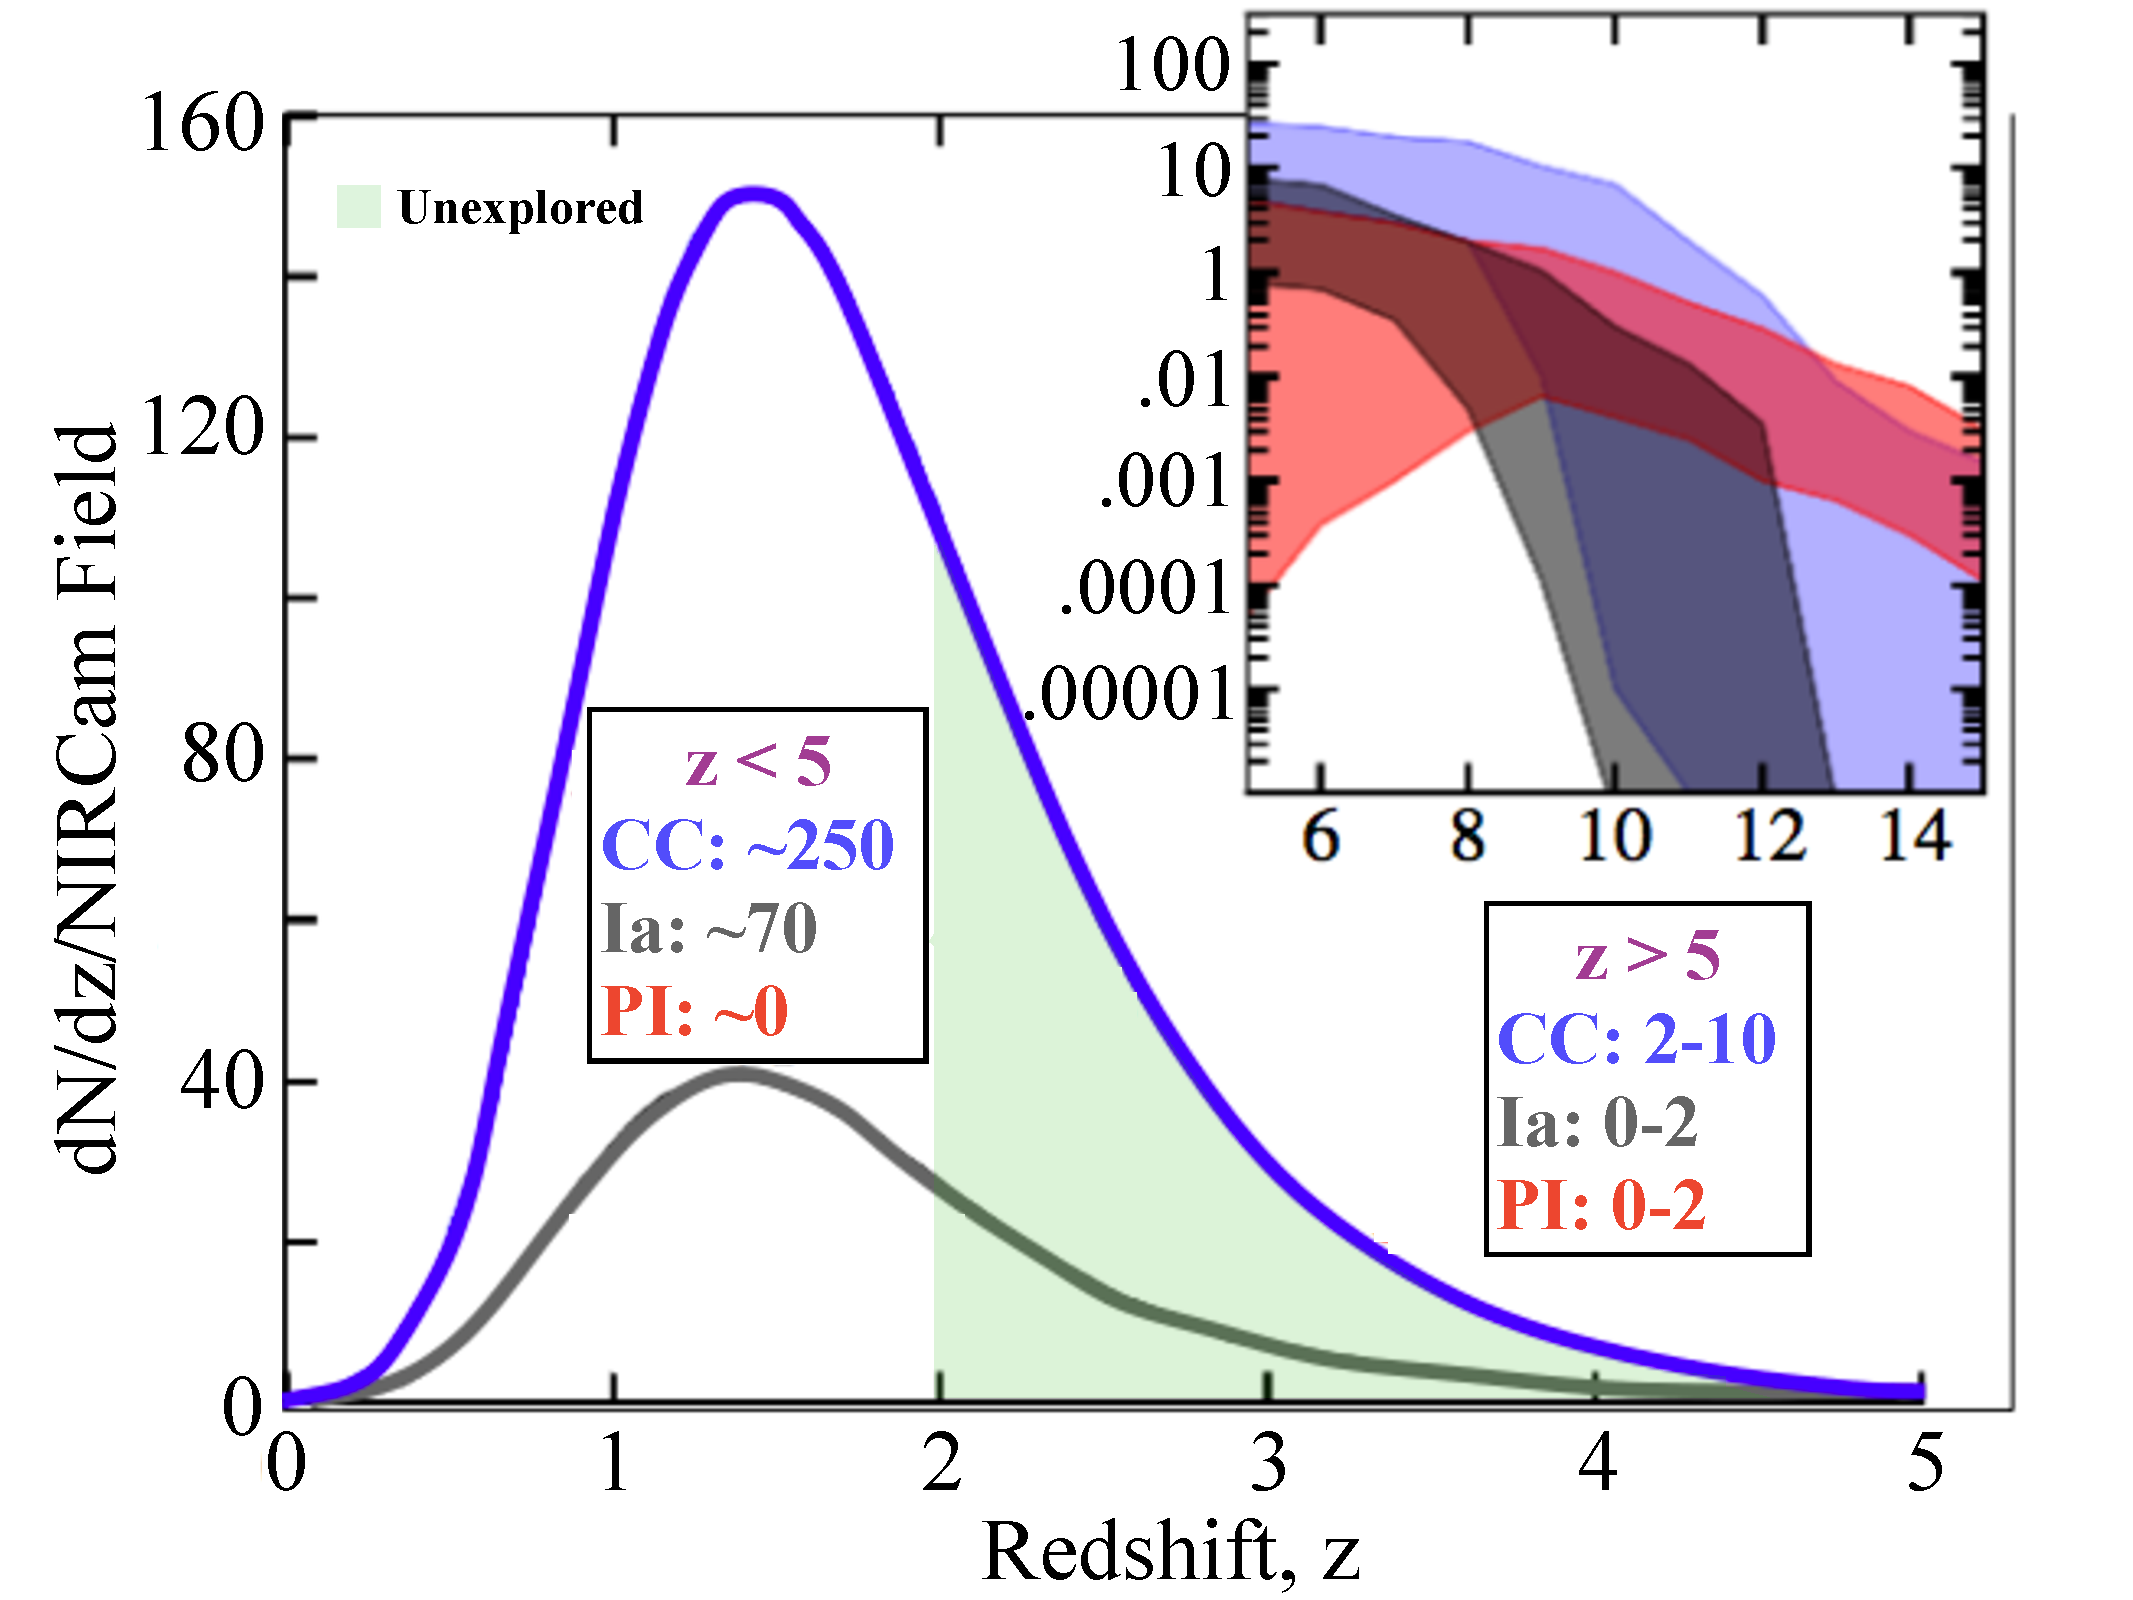
\includegraphics[height=.4\textwidth]{FIG/jwst_rates2}
%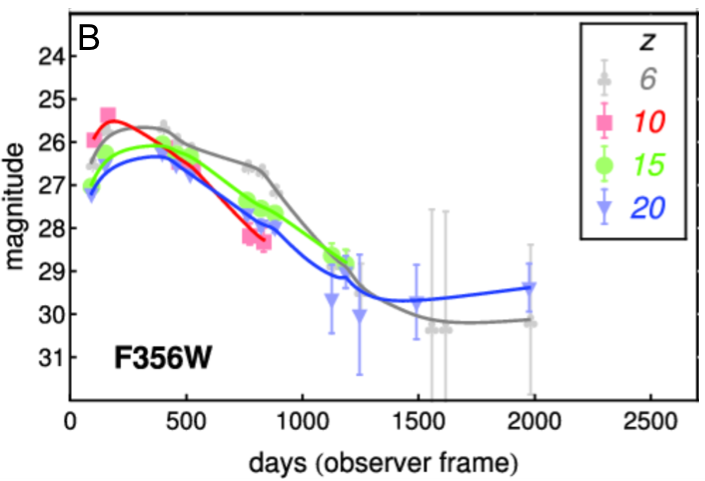
\includegraphics[height=.3\textwidth]{FIG/jwst_sim}
\caption{
\noindent\fontsize{10}{14}\selectfont
Projected SN yield from the JWST GTO 1176 program. We will
detect \textit{every} Type Ia SN that explodes in this field to z
$\lesssim5$ and 90$\%$ of all Core Collapse (CC) SNe to z $\simeq$
1.5, allowing the first high-z SN rate studies with an effectively
complete sample. The inset shows SN yield for $z>5$, where
observations of Type Ia and PI SNe are possible. The green region
represents redshifts above the most distant SN currently recorded,
suggesting that observations from the GTO will create a significant
catalog of the most distant SNe yet detected.}
\end{wrapfigure}

\noindent\underline{\textit{Research Plan}}:
1)Complete the python software package SNTD and write a publication
presenting its capabilities and validation. 2) Perform reanalysis of
SN Refsdal and SN iPTF16geu using SNTD, writing a second publication
presenting the more precise time delay measurements, detailing the
methodology required for these analyses, and obtaining a constraint on
$H_0$ from iPTF16geu. 3)Form a sample of high-z and lensed SNe from
HST surveys and JWST GTO, and write a publication with results such as
SFR and physical properties of SN progenitors in the early universe.

These \textbf{three publications}, as well as the vetting and
extensive use of the open-source SNTD package by the entire community
in future work with the next generation of space telescopes, will
be \textbf{clear measures of the success of this work.}

%Depending on the yield PISN

\noindent\underline{\textit{Broader Impacts}}:
I will use my previous STEM outreach experiences (see personal
statement) to \textbf{increase the participation of young students in
astronomy and other STEM fields from my neighborhood in Columbia, SC,
where 88$\%$ of the residents are underrepresented minorities in
STEM.}  My research is a terrific gateway into STEM because it is
naturally exciting and interesting: space telescopes, exploding stars,
and gravitational lensing are surefire topics to capture the attention
and imagination of a young learner. I have already created a plan with
the \textit{Lyon Street Community After School Program} leader that
will include taking the kids to our local University observatory, and
leading them through a series of exciting and educational astronomical
exercises over the course of the year. I will have each student choose
and carry out an astronomy project within our neighborhood, such as
monitoring sunspots to measure the rotation of the sun, and present
their results to the community. By teaching the students and engaging
their parents via the research projects and presentations, this outreach
program will \textbf{ encourage higher learning in STEM, and increase
public scientific literacy and public engagement with STEM}.

\noindent\fontsize{10}{14}\selectfont
[1]Kelly, P. L., et al. 2015, Science, 347, 1123 [2]Goobar, A., et
al. 2016, arXiv:1611.00014v1 [3]Oguri, M., $\&$ Marshall, P. J. 2010,
MNRAS, 405, 2579 [4]Rodney, S. A., et al. 2015, ApJ, 811,70
[5]Rodney, S. A., et al. 2016, ApJ, 820, 50 [6]Suyu, S. H., et
al. 2014, ApJ, 788, L35 [7]Kolatt, T. S., $\&$ Bartelmann, M. 1998,
MNRAS, 296, 763 [8]Oguri, M., $\&$ Kawano, Y. 2003, MNRAS, 338, L25
[9]Whalen, D. J., et al. 2013, arXiv:1312.6330 [10]de Souza, R. S., et al. 2013, MNRAS, 436, 1555
\pagebreak
%plan with after-school program leader. presenting to community members-->existing real connections in community. Appropriate scope for solitary grad student. 

%measure of success:


%Growing sample of gravitationally lensed publically available where tools would be available (rubin & haden-''The discovery of a gravitationaly lensed supernova Ia at redshift 2.22)

%First paragraph-->make it more of a thesis sentence at the end, instead of there is no current package. maybe also jwst high redshift sne for me to analyze.

%Figure from proposal (6a), measuring high redshift supernova rates of all types

%1. does a sn at a redshift of 4 (CC Or Ia) look the same as a sn at 1 or 2?

%2. if we measure the rate of ia and cc sne to a redshift of 3 and 4, what do the progenitor star systems look like?

%3. cosmology with type ia sne (adding to hubble diagram)

%First measure of sfr beyond redshift of 2

